\subsection{Introduction}
\textbf{Synchronized activity among neurons} occurs in many brain areas and there are evidences
suggesting that it is relevant for information processing, and, especially, for sensory
processing, cognition and sleep. Patters of reverberating synchronized activity are
believed to reflect neuronal representations of cognitive processes and stored
memories. This kind of synchronized activity is also observed
\textit{in vitro}.\\
A \textbf{network burst (NB)} can be described as a synchronized bursting event involving most units of the network, thus implying that several channels are exhibiting bursting activity at the same time.
\begin{figure}[H]
    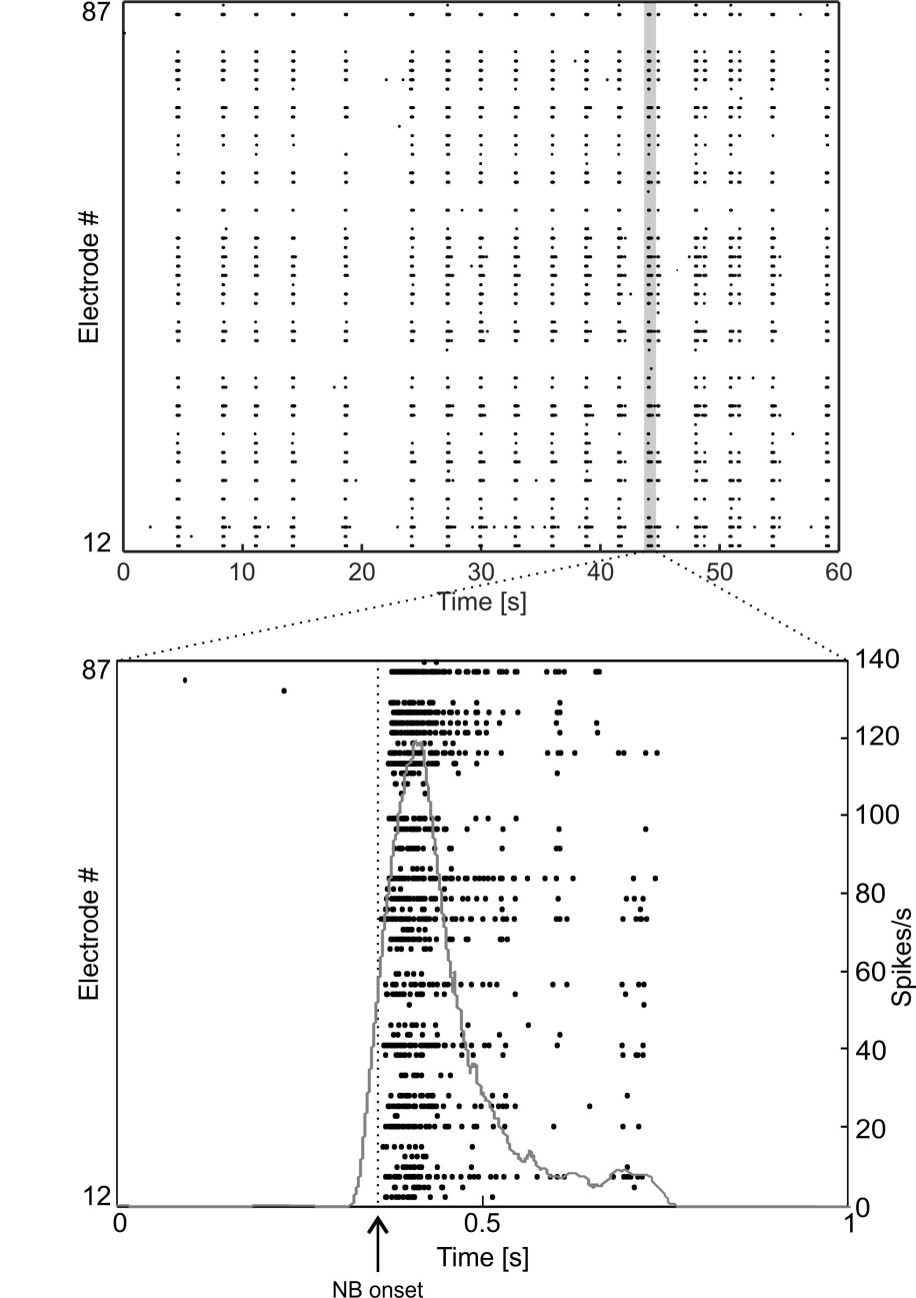
\includegraphics[scale=0.28]{7_1}
    \centering
\end{figure}

\paragraph{LFPs vs MUA}
Network bursting closely reminds to the \textit{UP} and \textit{DOWN} states 
of the \textit{in vivo} cerebral cortex during slow-wave sleep. 
In addition, spontaneous network bursting activity is also easily
noticed in the developing brain, as it is thought to play a key role in
ontogeny (i.e. the origination and development of an organism)
of a neuronal network.\\
In general, it is possible to individuate 6 types of waves, each one described by a typical frequency range:
\begin{itemize}
    \item \textbf{Delta}: \(0.5-4\,Hz\)
    \item \textbf{Theta}: \(4-8\,Hz\)
    \item \textbf{Alpha}: \(8-11\,Hz\)
    \item \textbf{Beta}: \(11-30\,Hz\)
    \item \textbf{Low Gamma}: \(30-55\,Hz\)
    \item \textbf{High Gamma}: \(55-80\,Hz\)
\end{itemize}
\subsection{Example: A Step Into Sleep Physiology}
In mammals and birds, sleeping activity is divided into pretty much different
phases, according to the characteristics exhibited by the brain activity:
\begin{itemize}
    \item \textbf{Rapid Eye Movement (REM):} this phase is also known as \textit{paradoxical
          sleep}. It is characterized by rapid eye movements as well as a rapid low-voltage EEG, similar to the awake state. 
    \item \textbf{Non-Rapid Eye Movement (NREM):} this broad category keeps together
          all the phases where the neuronal activity is considerably different with respect to the awake state. Different NREM stages can be individuated according to the activities:
          \begin{itemize}
              \item \textbf{N1:} it refers to the transition of the brain from alpha waves
                    (awake state with \(f\simeq8-10\,Hz\)) towards theta waves (\(f\simeq4-7\,Hz\)). This stage is often called \textit{drowsy sleep}.
              \item \textbf{N2:} it is characterized by a phenomenon denominated sleep
                    spindles (i.e. bursts of activity), displaying a higher frequency range (\(11-16\,Hz\)). Spindles are related to plasticity and memory. Another typical phenomenon occurring in this stage is K-complexes. 
              \item \textbf{N3:} this stage is commonly denominated \textit{deep sleep} (or \textit{slow-wave sleep}) and it is
                    characterized by the presence of delta waves (at least \(20\%\) of the
                    overall activity) ranging from \(0.5\,Hz\) to \(2\,Hz\). Notice that delta waves exhibit high peak-to-peak voltages (\(>75\,\mu{V}\)).
              \item \textbf{N4:} this stage is usually described as a state in which slow
                    delta waves overcome the \(50\%\) threshold on the total brain oscillatory
                    activity. It is sometimes considered together with stage N3.
          \end{itemize}
\end{itemize}
\begin{figure}[H]
    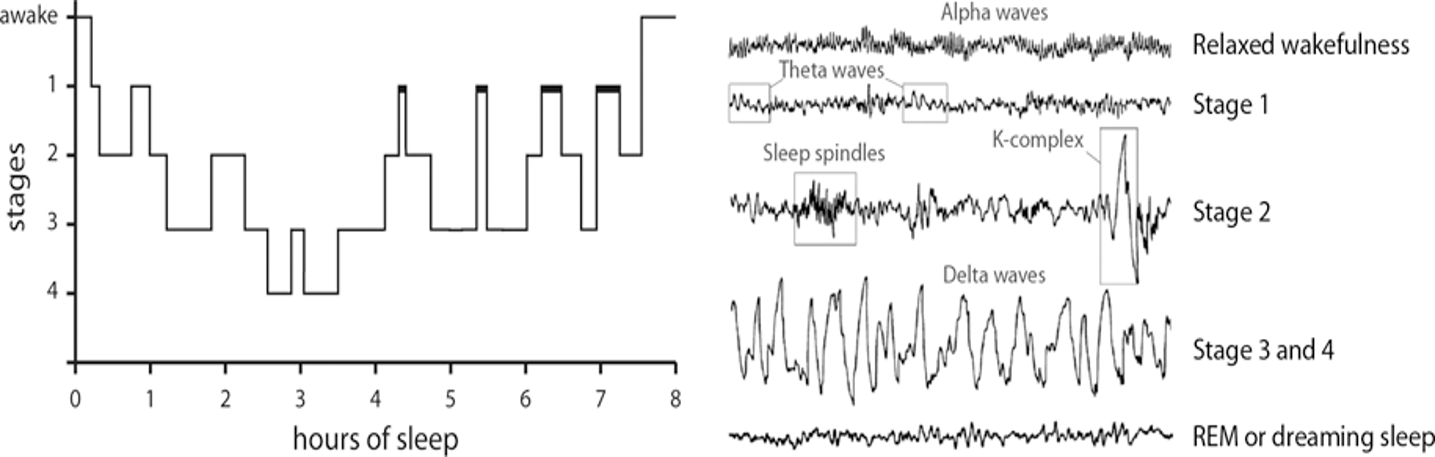
\includegraphics[scale=0.70]{7_2}
    \centering
\end{figure}
There is evidence that network bursting activity is strictly related to the delta waves 
typical of deep sleep, because the periodicity seems to be compatible with the waves during this stage.
\subsection{Network Burst Detection}
In order to detect network bursts, it is necessary to be able to recognize synchronous
increases in the network activity. A number of algorithms have been developed to
solve such a task.
\subsubsection{The Van Pelt algorithm}
Network bursts are short episodes of synchronized firing among many recording sites. They are not
exclusively described by increased firing rates at individual sites, but also by an
increase of the number of active sites.\\ 
The Van Pelt algorithm consists in dividing the time
axis into a number of small bins and computing the product between the number of
active sites (i.e. the recording channels showing firing activity) and the total
number of spikes at these sites. In case of uncorrelated spiking activity among
the sites, this product won't significantly differ from the total spike count, however
it raises sharply as soon as the firing becomes synchronized. The time point at
which the product reaches its maximum value is used to
define a center-of-mass-based time center of the network burst.
\begin{figure}[H]
    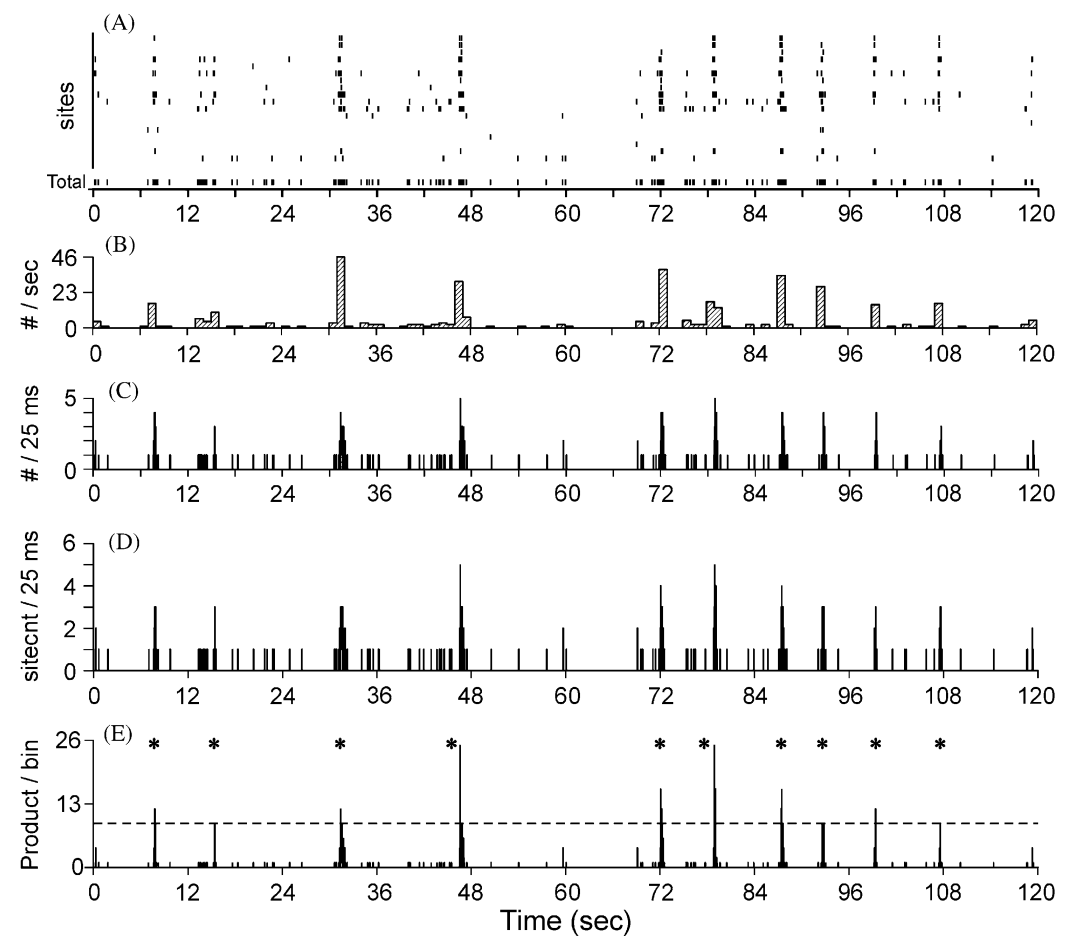
\includegraphics[scale=0.6]{7_3}
    \centering
\end{figure}
\pagebreak
The last figure shows the network burst detection procedure:
\begin{itemize}
    \item[(A)] The time points of spikes at the different recording sites of
          a multi-electrode array. The lowest trace shows the total spike train for all
          the sites.
    \item[(B)] A total network firing rate plot with time bins of \(1\,s\).
    \item[(C)] A total network firing rate plot with time bins of \(25\,ms\).
    \item[(D)] A plot of the number of active sites with time bins
          of \(25\,ms\).
    \item[(E)] A plot of the product of total number of spikes and the
          number of active sites, calculated per \(25\,ms\) time bins. The dashed line
          represents a threshold to overcome to identify an actual network burst, which
          are individuated by a star.
\end{itemize}
Having the raster plot, a division with bins of \(25\,ms\) can be performed. This can tell if there are times in the recording with an increased activity. Then, an improvement is to consider not only the spike count, but also how many channels are active in the same bin. It should be better to avoid to have 1 channel with 1 burst and 20 with 0 bursts, but if there is a channel with many bursts, then it should be considered in a different way.
\subsubsection{The LogISI method}
This technique requires that burst detection has been performed for every
recording channel. Then, a burst event train for each channel is derived, where
bursts are described as single point events, disregarding every information about
their duration. These points for all the sites are then projected onto the same axis.
At this point, burst detection is performed again on this new axis, allowing
to look for time periods with an increased bursting activity on several channels (thus
synchronized). Therefore, this algorithm consists in an iterative application of burst detection procedures.\\
Notice that the minimum number of intra-burst spikes for the cumulative
burst event train can be intended as the minimum number of active channels required
to detect a network burst event, usually set as the \(20\%\) of the total number of
recording sites.
\begin{figure}[H]
    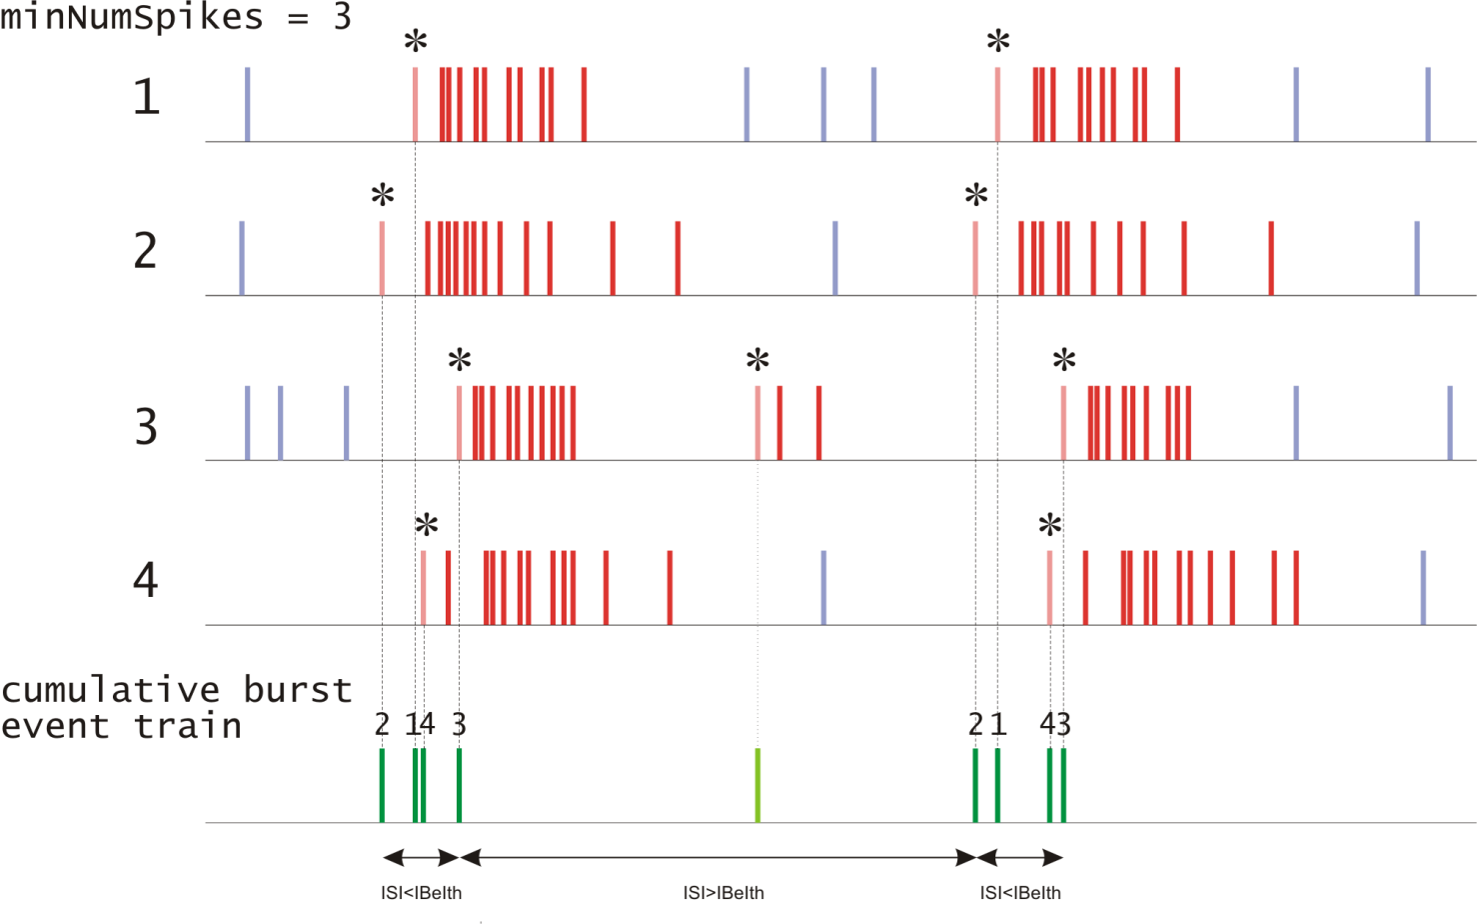
\includegraphics[scale=0.65]{7_4}
    \centering
\end{figure}

\subsection{Metrics}
Some of the most relevant metrics to characterize network bursting are reported
in the following.
\subsubsection{The Burstiness Index}
The burstiness index (\(BI\)) is a metric, empirically derived by D. A. Wagenaar in order to assess the burstiness
of a neuronal network with just one number. From experiments, it has been noticed that,
in general, the overall time occupied by network bursts in a whole recording is
always less than \(15\%\) of the total duration, and this factor has been taken as an
assumption for the computation of constants employed to derive the burstiness
index.\\ 
The computation steps are reported here:
\begin{enumerate}
    \item Divide a 5 minutes recording into time bins (each 1 second long), obtaining 300 of them.
    \item Count the total number of spikes for each bin, across all the recording sites.
    \item Compute the fraction of the total number of spikes contained in the \(15\%\)
          of bins with the largest counts, indicated as \(f_{15}\).
          \begin{itemize}
              \item If the firing rate is tonic, then \(f_{15}\) is expected to be close to \(0.15\).
              \item If a recording is bursty, it is more likely that most of the spikes will
                    be contained in bursts, resulting in \(f_{15}\) close to \(1\).
          \end{itemize}
    \item Compute the \textbf{burstiness index} normalized between \(0\) and \(1\) as
          \begin{align*}
              BI = \frac{f_{15}-0.15}{0.85}
          \end{align*}
\end{enumerate}
\subsection{Major Burst Leaders}
Each network burst spreads through the recording sites according to a specific
spatio-temporal pattern, resulting in a precise sequence of electrodes activation.
Major Burst Leaders (MBLs) are the privileged nodes in the network that consistently
fire earlier than the others at the onset of the network bursts. It is critical to
individuate them, as they play the role of leaders of the synchronized bursting
activity. The pool of MBLs is stable across hours, although the leadership frequency of individual channels may vary.\\
In general, MBLs are not unique. The first firing neuron in the network burst is called \textbf{Burst Leader} (BL) and, looking at the definition, 
it is intuitive the fact that the BL is unique, even if it may change in time, being one of the MBLs but not always the same.
\newpage
Each node is given a certain leadership score, as shown in the following figure, according
to its relevance in the initiation of a bursting event. If such score overcomes a
certain threshold (indicated by the dotted line), then the node is identified as
one of the MBLs.
\begin{figure}[H]
    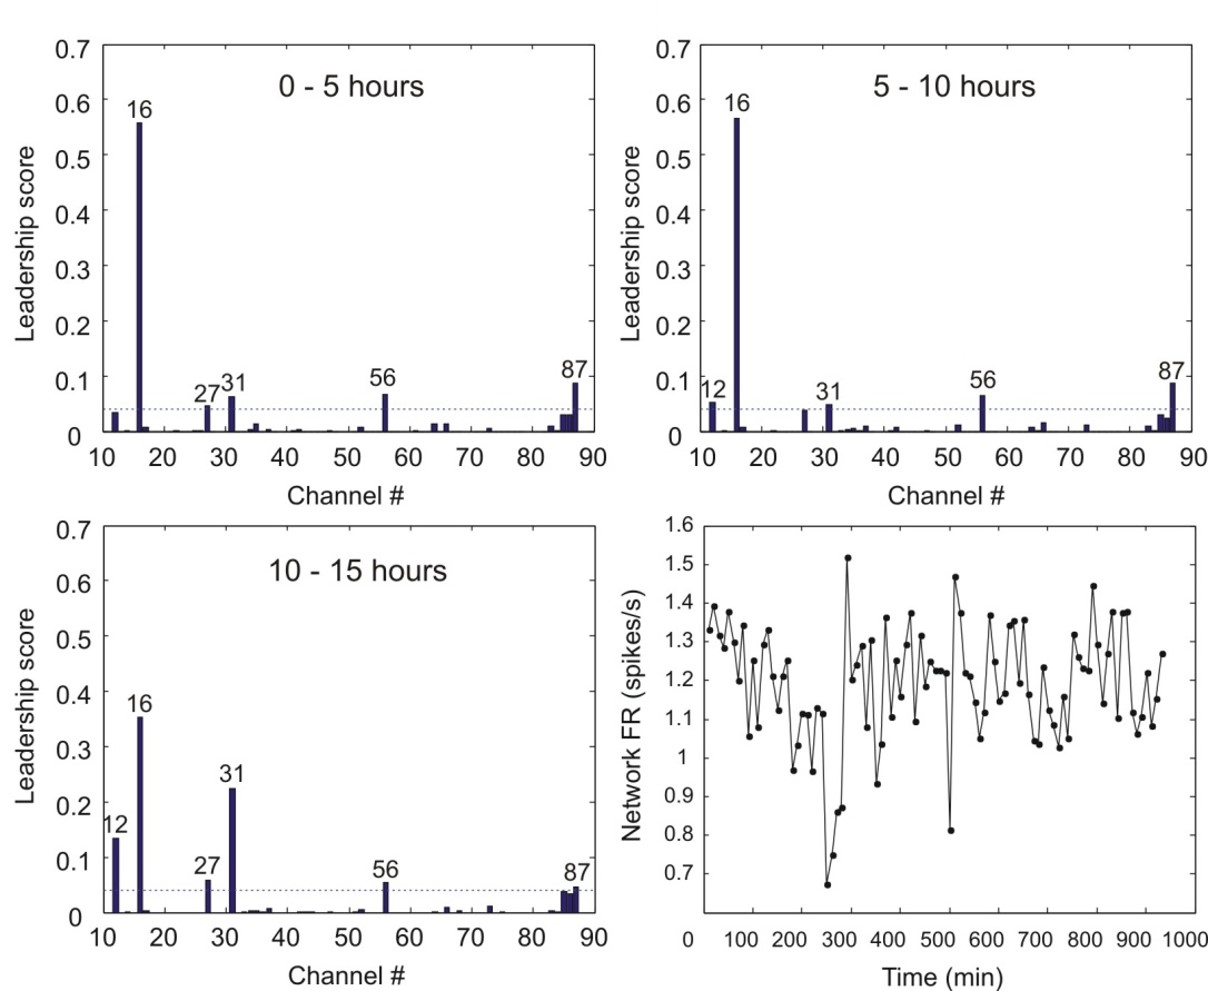
\includegraphics[scale=0.7]{7_5}
    \centering
\end{figure}
Another crucial phenomenon is the recruitment of MBLs. In fact,
as soon as MBLs are activated, they recruit other MBLs in the network burst pathway, where by recruitment it is meant
the activation of other nodes in order to facilitate the initiation of a network burst.
In addition, MBLs are involved in network bursting activity with a higher reliability
than other common nodes (\(>90\%\)).
\begin{figure}[H]
    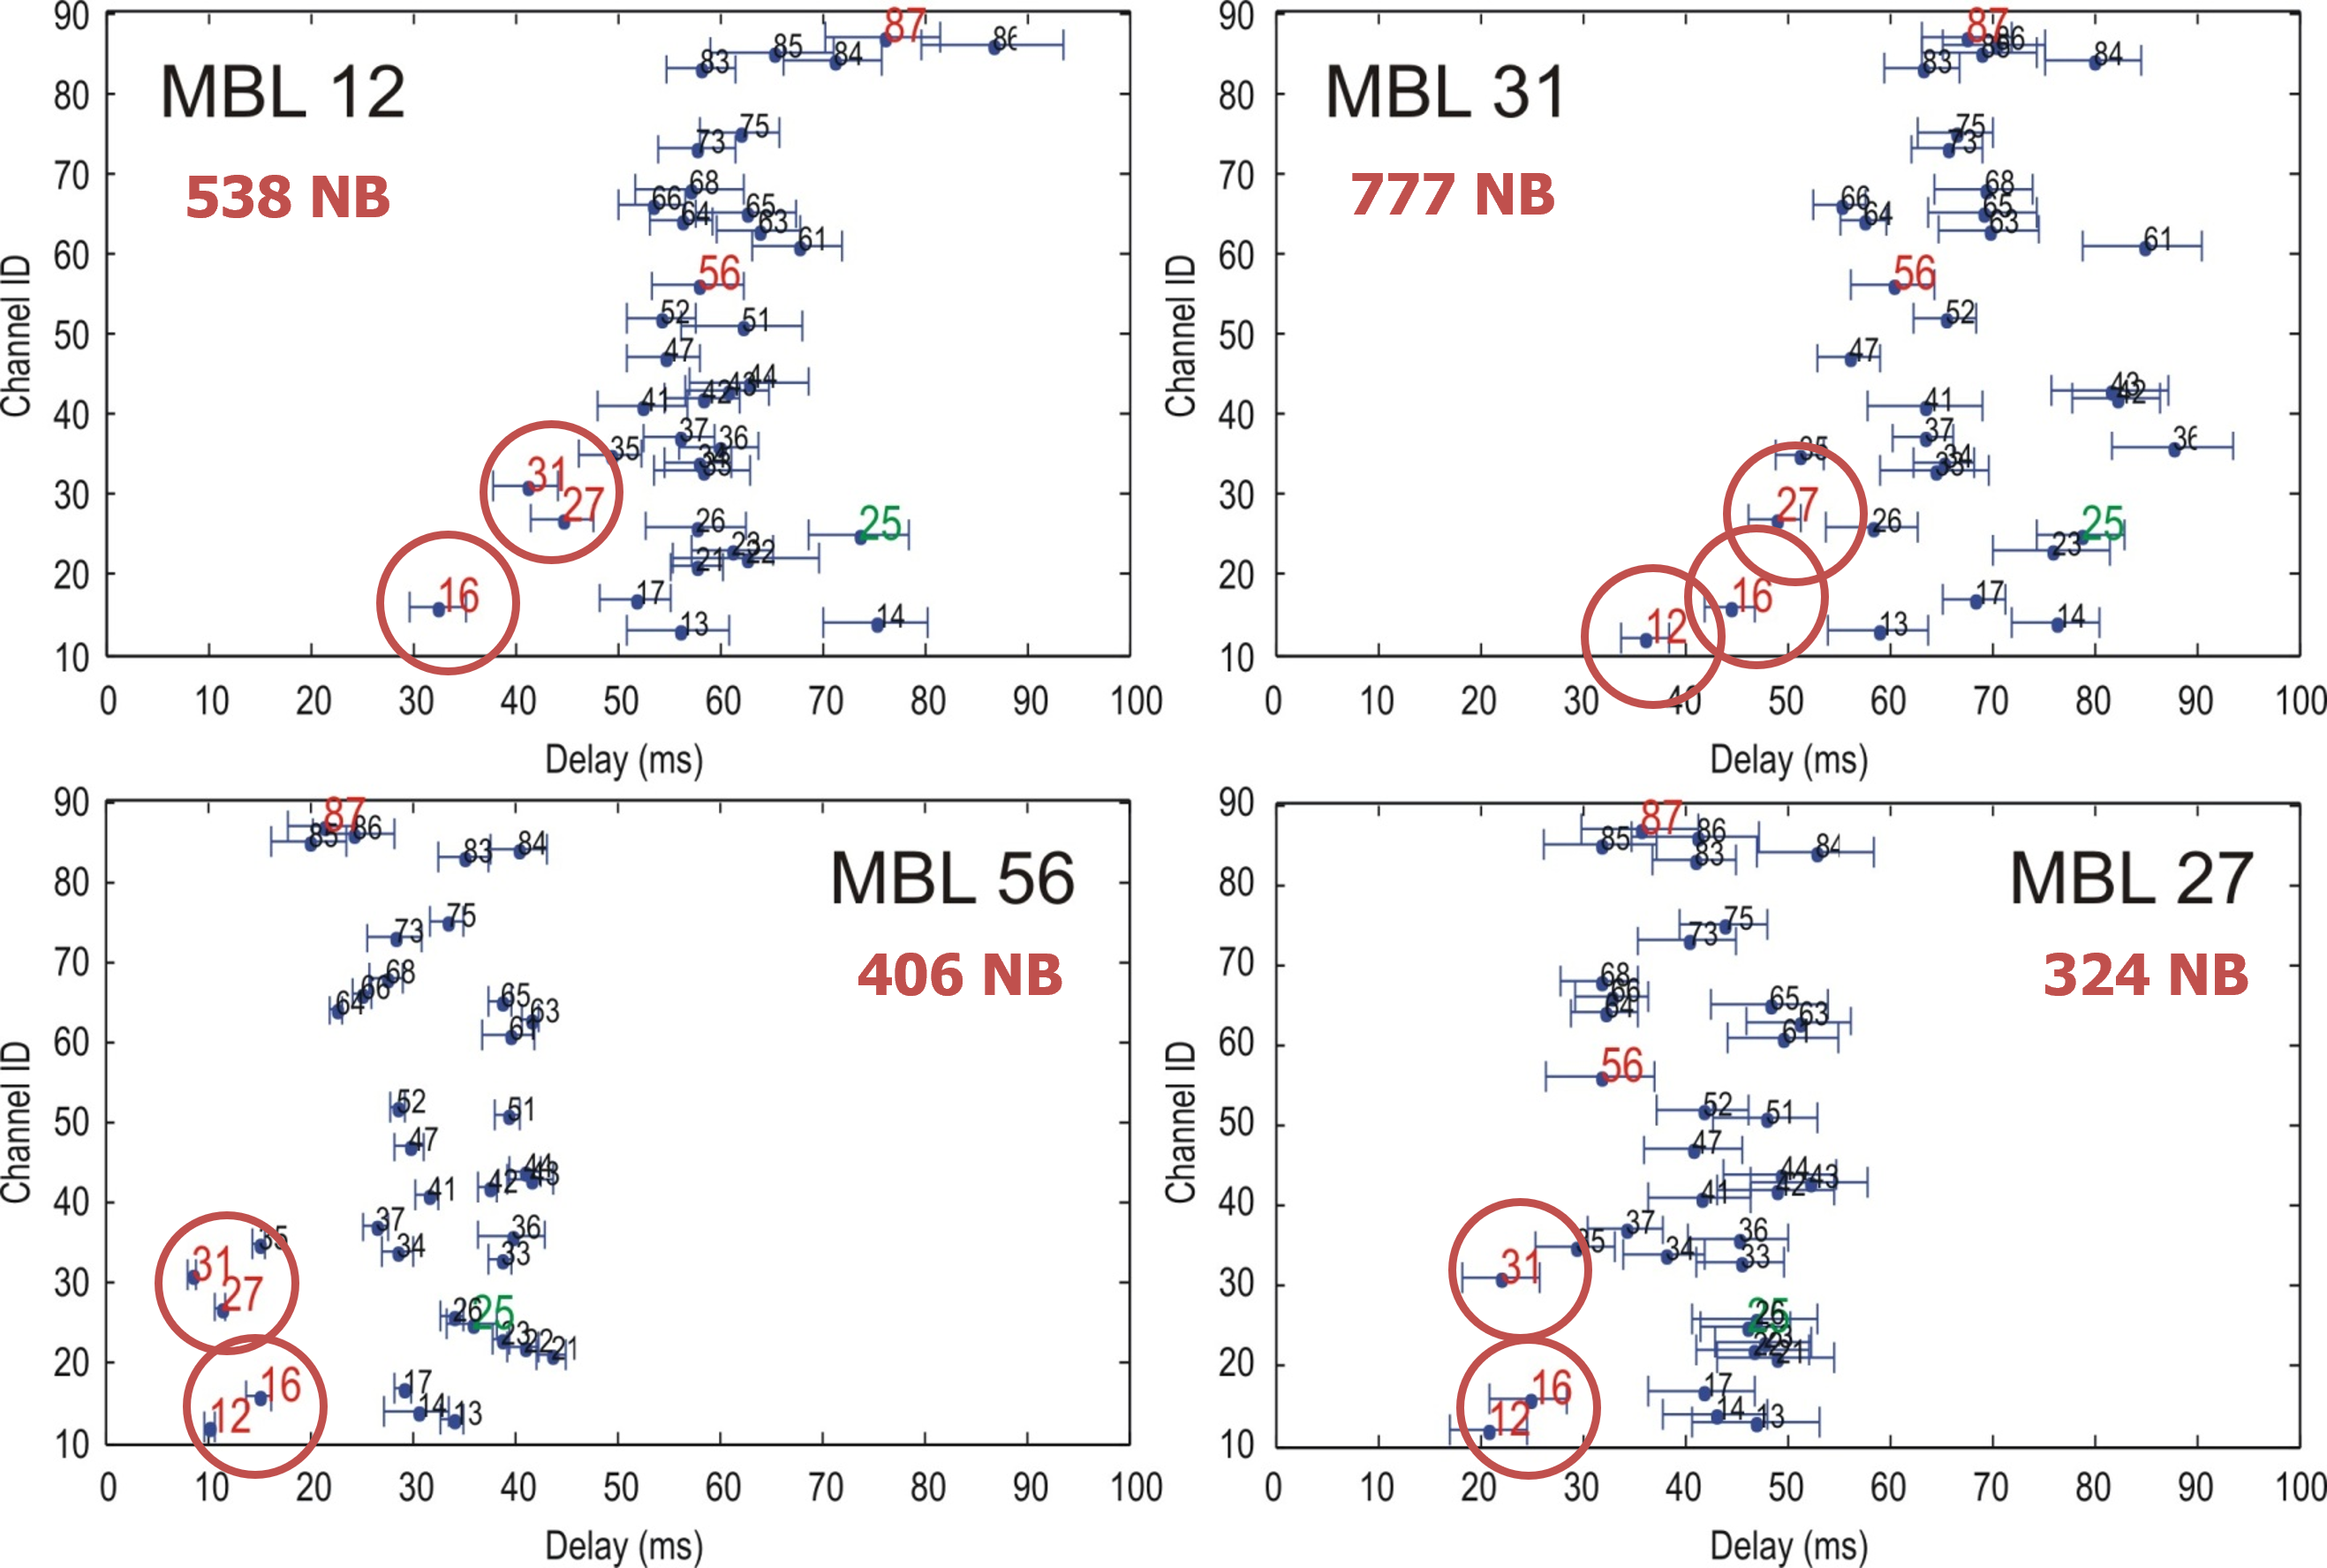
\includegraphics[scale=0.65]{7_6}
    \centering
\end{figure}
At this point, one might wonder if MBLs represent the most active channels in terms
of spikes. Although no correlation between the leadership score and the fraction of
spikes outside network bursts has been assessed, it has been observed that almost
all MBLs have a sustained spiking activity, with an average firing rate higher than
the network average. Moreover, it seems that their response to electrical stimulation
is indeed stronger and faster than the one of common neurons.
\begin{figure}[H]
    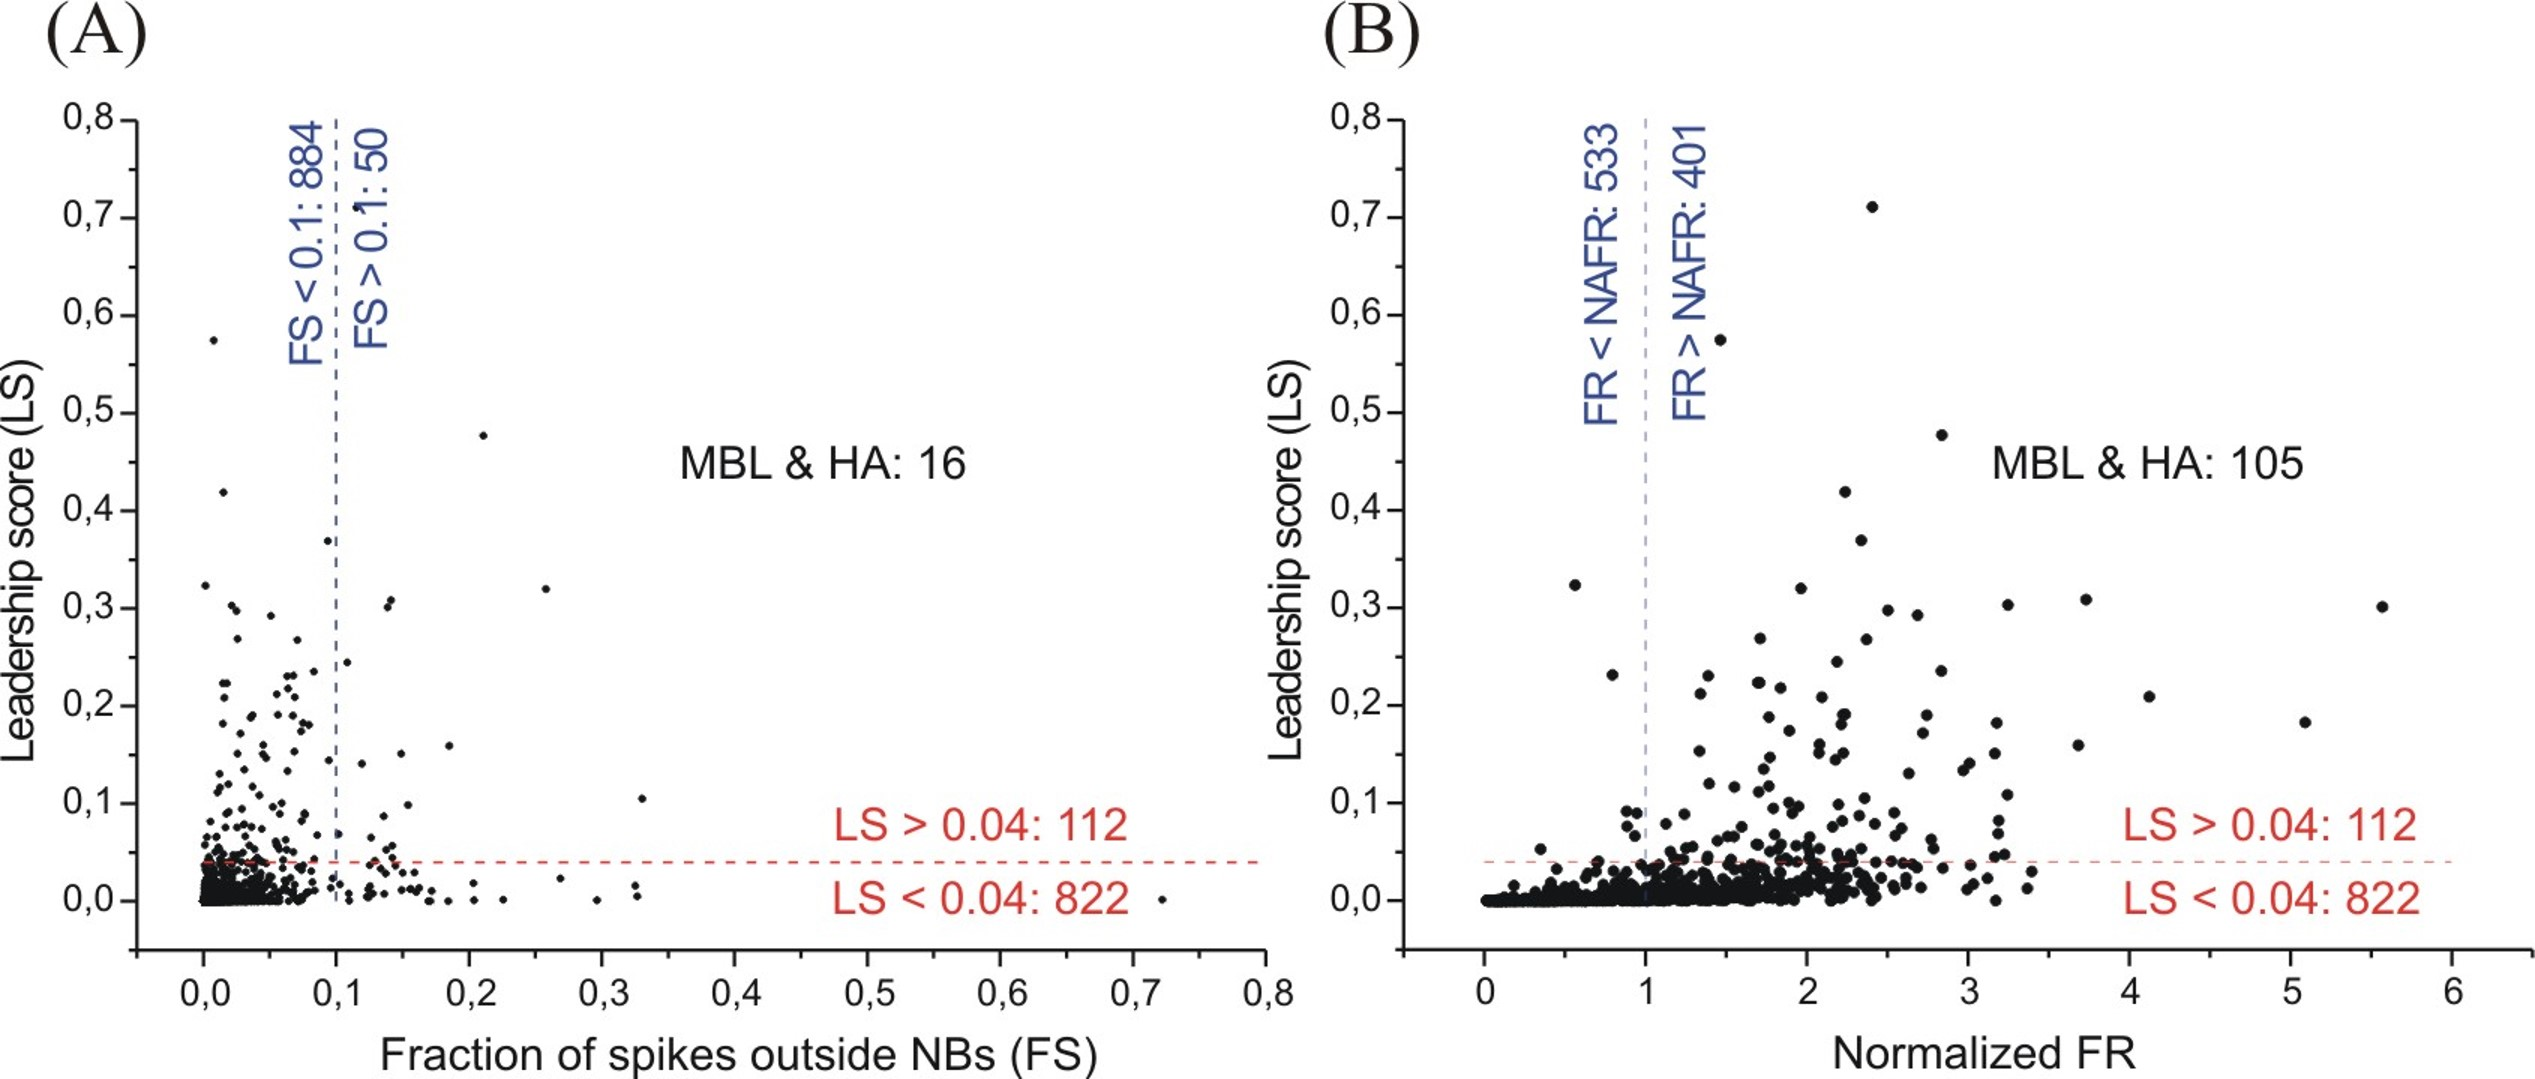
\includegraphics[scale=0.7]{7_7}
    \centering
\end{figure}
A possible interpretation of this phenomenon could be that MBLs receive a large number
of incoming excitatory connections, acting as \textbf{network hubs}, integrating
several inputs and redistributing them to the network.